To check the validity and robustness of the FNP lepton estimate, 
the distributions of several discriminating variables in data are compared 
with the predicted background after various requirements on the number of jets and $b$-jets. 
Examples of such distributions are shown in Figure~\ref{fig:Bkg_distribs}, 
and illustrate that the data are described by the prediction within 
uncertainties. 
%The apparent disagreement 
%for \meff\ above 1 TeV in Figure~\ref{fig:VRmeff2} is covered by the large theory uncertainty for the diboson background, which is not shown 
%but amounts to about 30\% for \meff\ above 1 TeV.

\begin{figure}[th!]
\centering
\begin{subfigure}[t]{0.49\textwidth}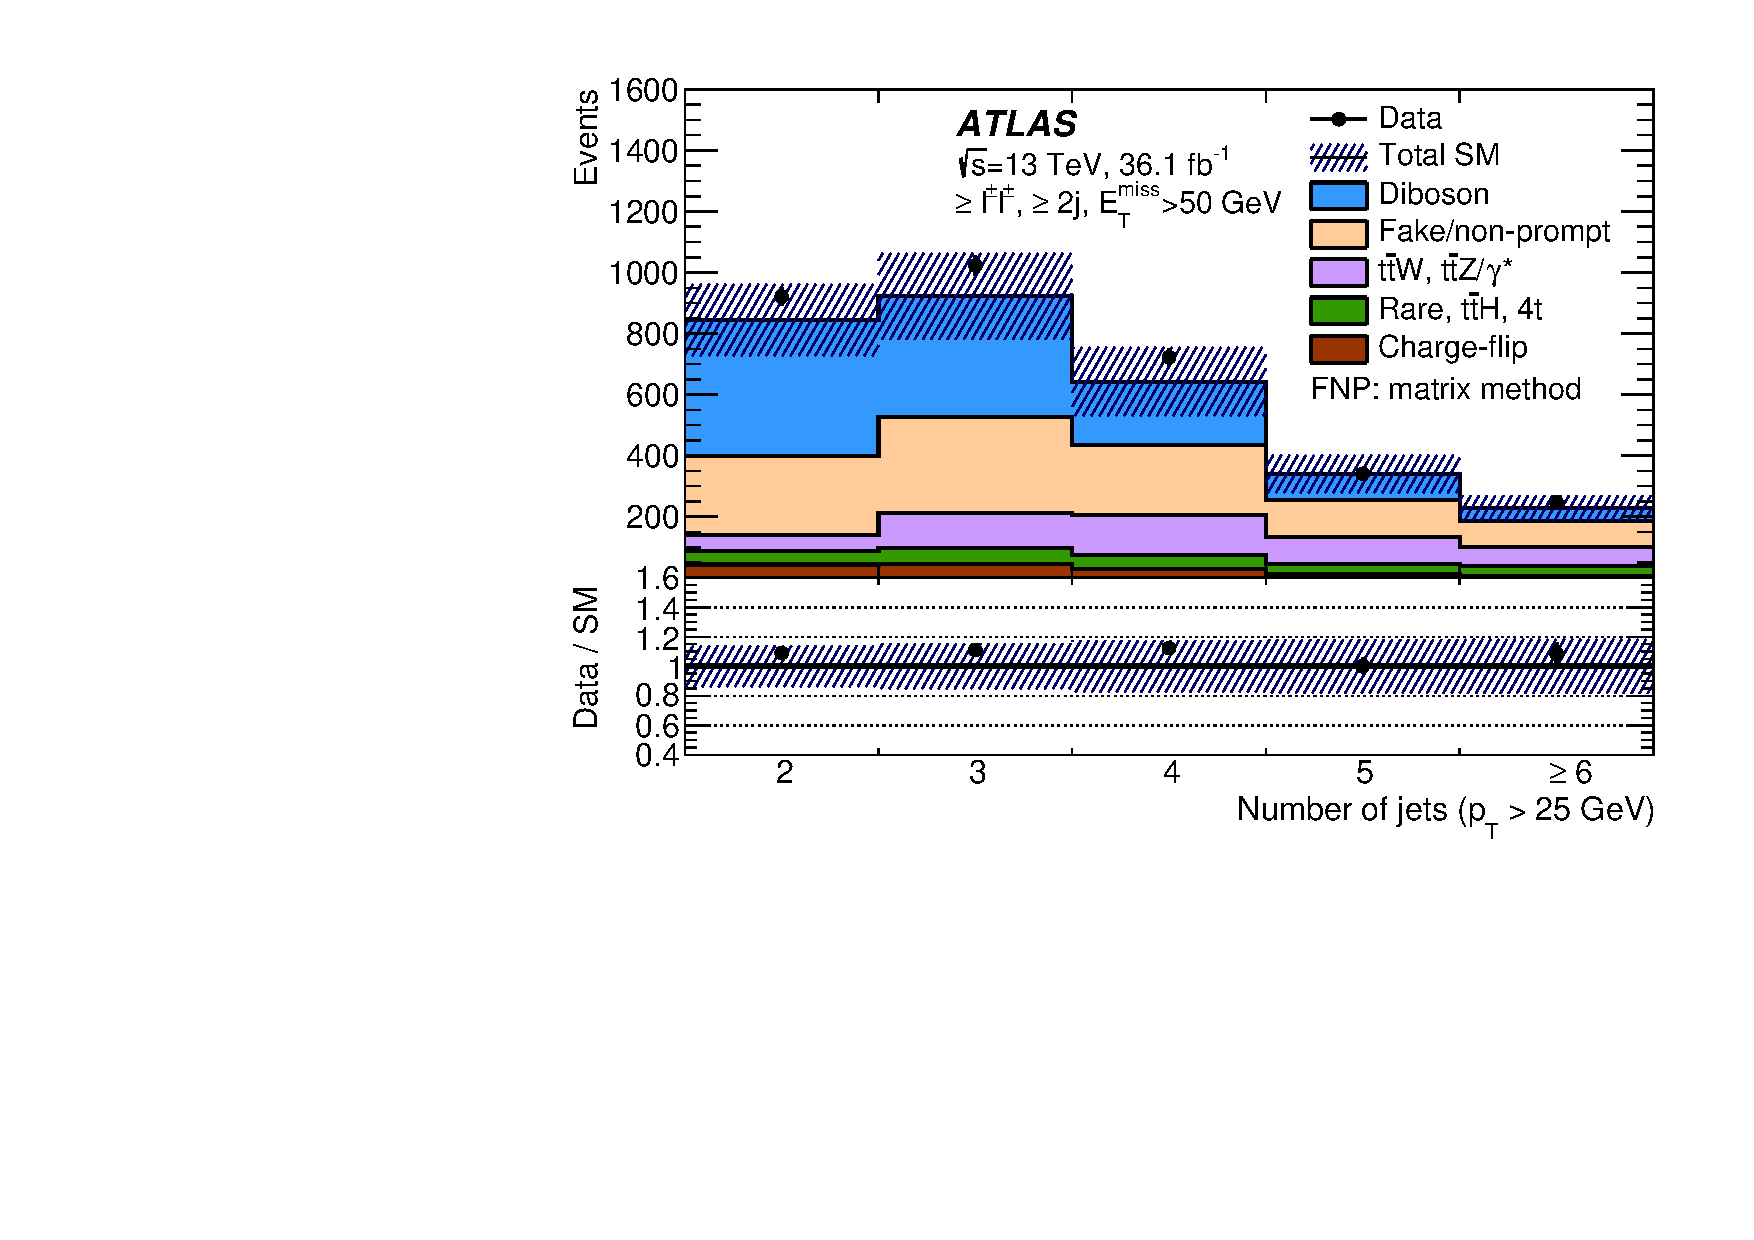
\includegraphics[width=\textwidth]{PAPER_DILEP_2JMET50_njets25}\caption{}\label{fig:VRnj}\end{subfigure}
\begin{subfigure}[t]{0.49\textwidth}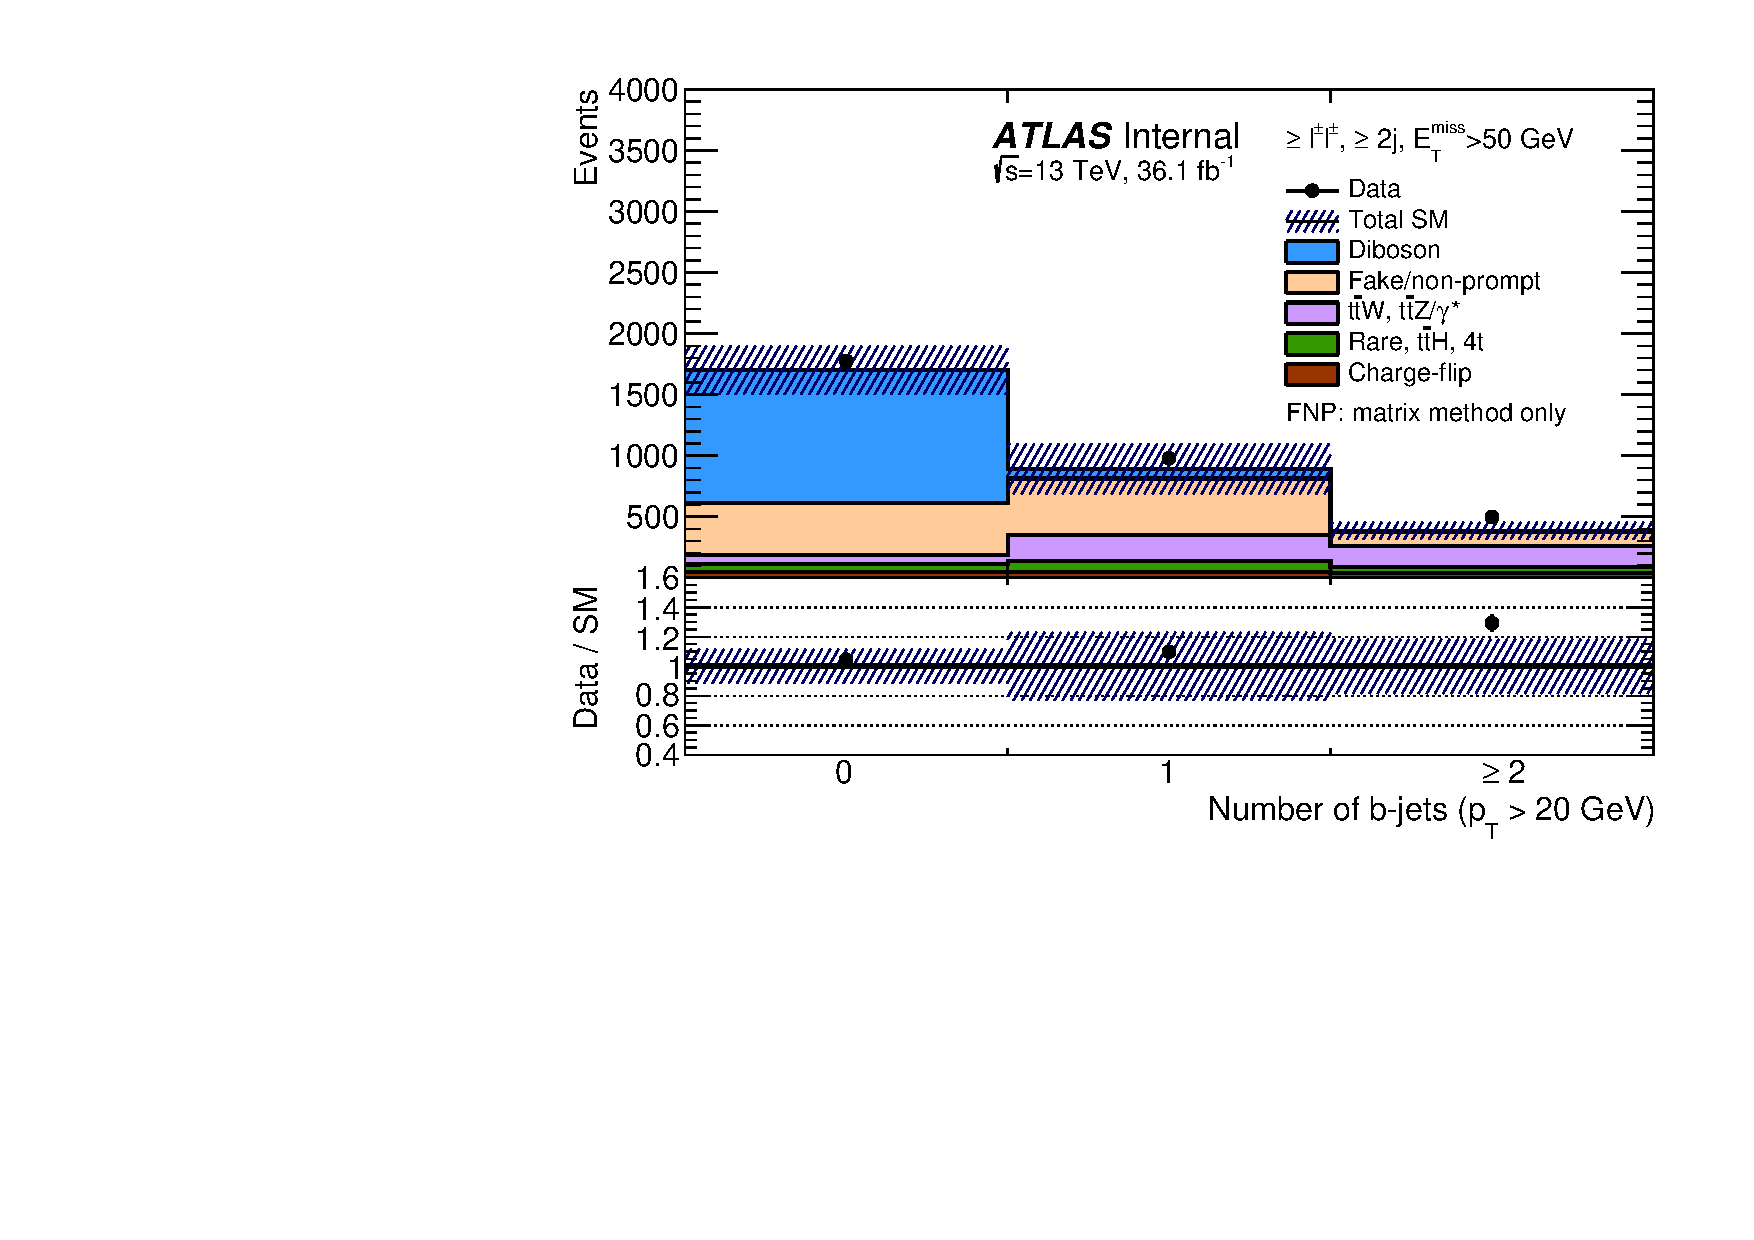
\includegraphics[width=\textwidth]{PAPER_DILEP_2JMET50_nbjets}\caption{}\label{fig:VRnb}\end{subfigure}
\begin{subfigure}[t]{0.49\textwidth}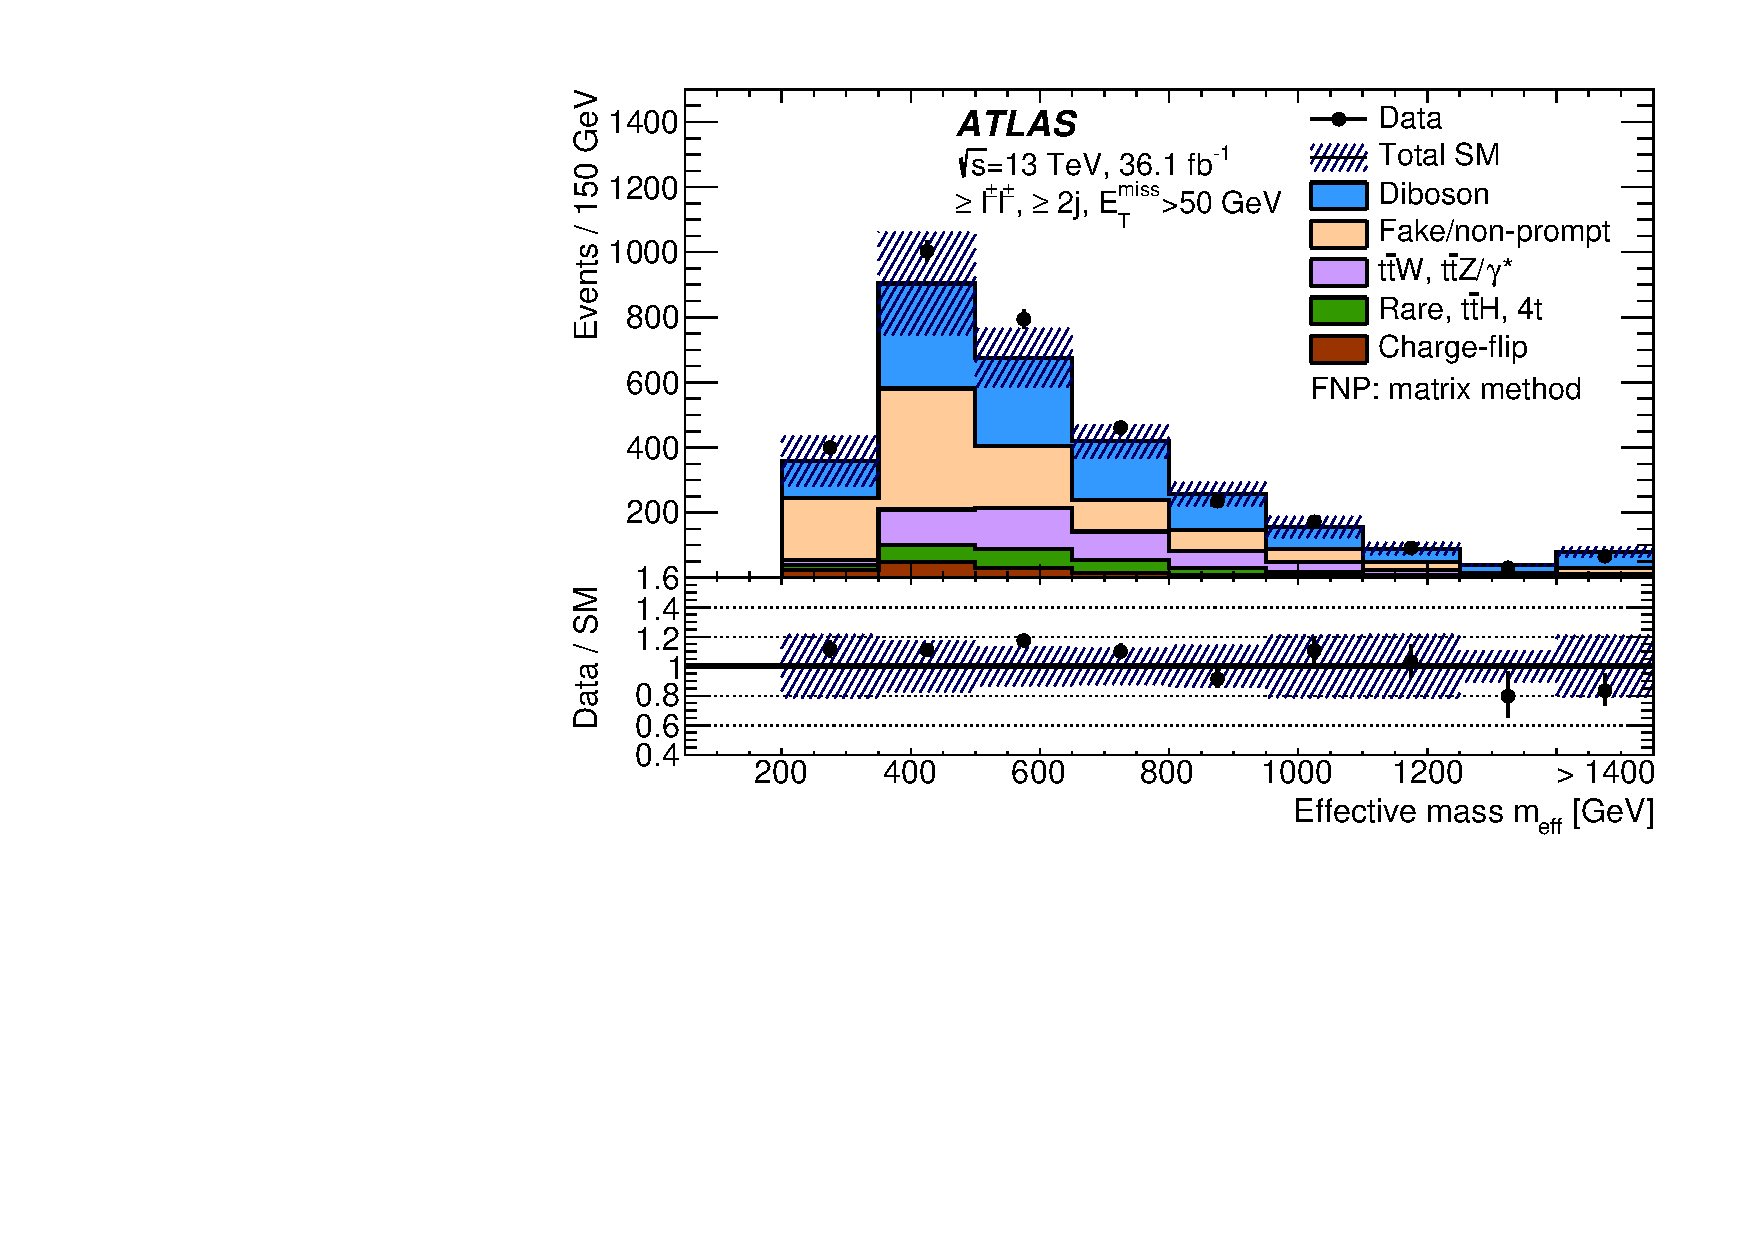
\includegraphics[width=\textwidth]{PAPER_DILEP_2JMET50_meff}\caption{}\label{fig:VRmeff1}\end{subfigure}
\begin{subfigure}[t]{0.49\textwidth}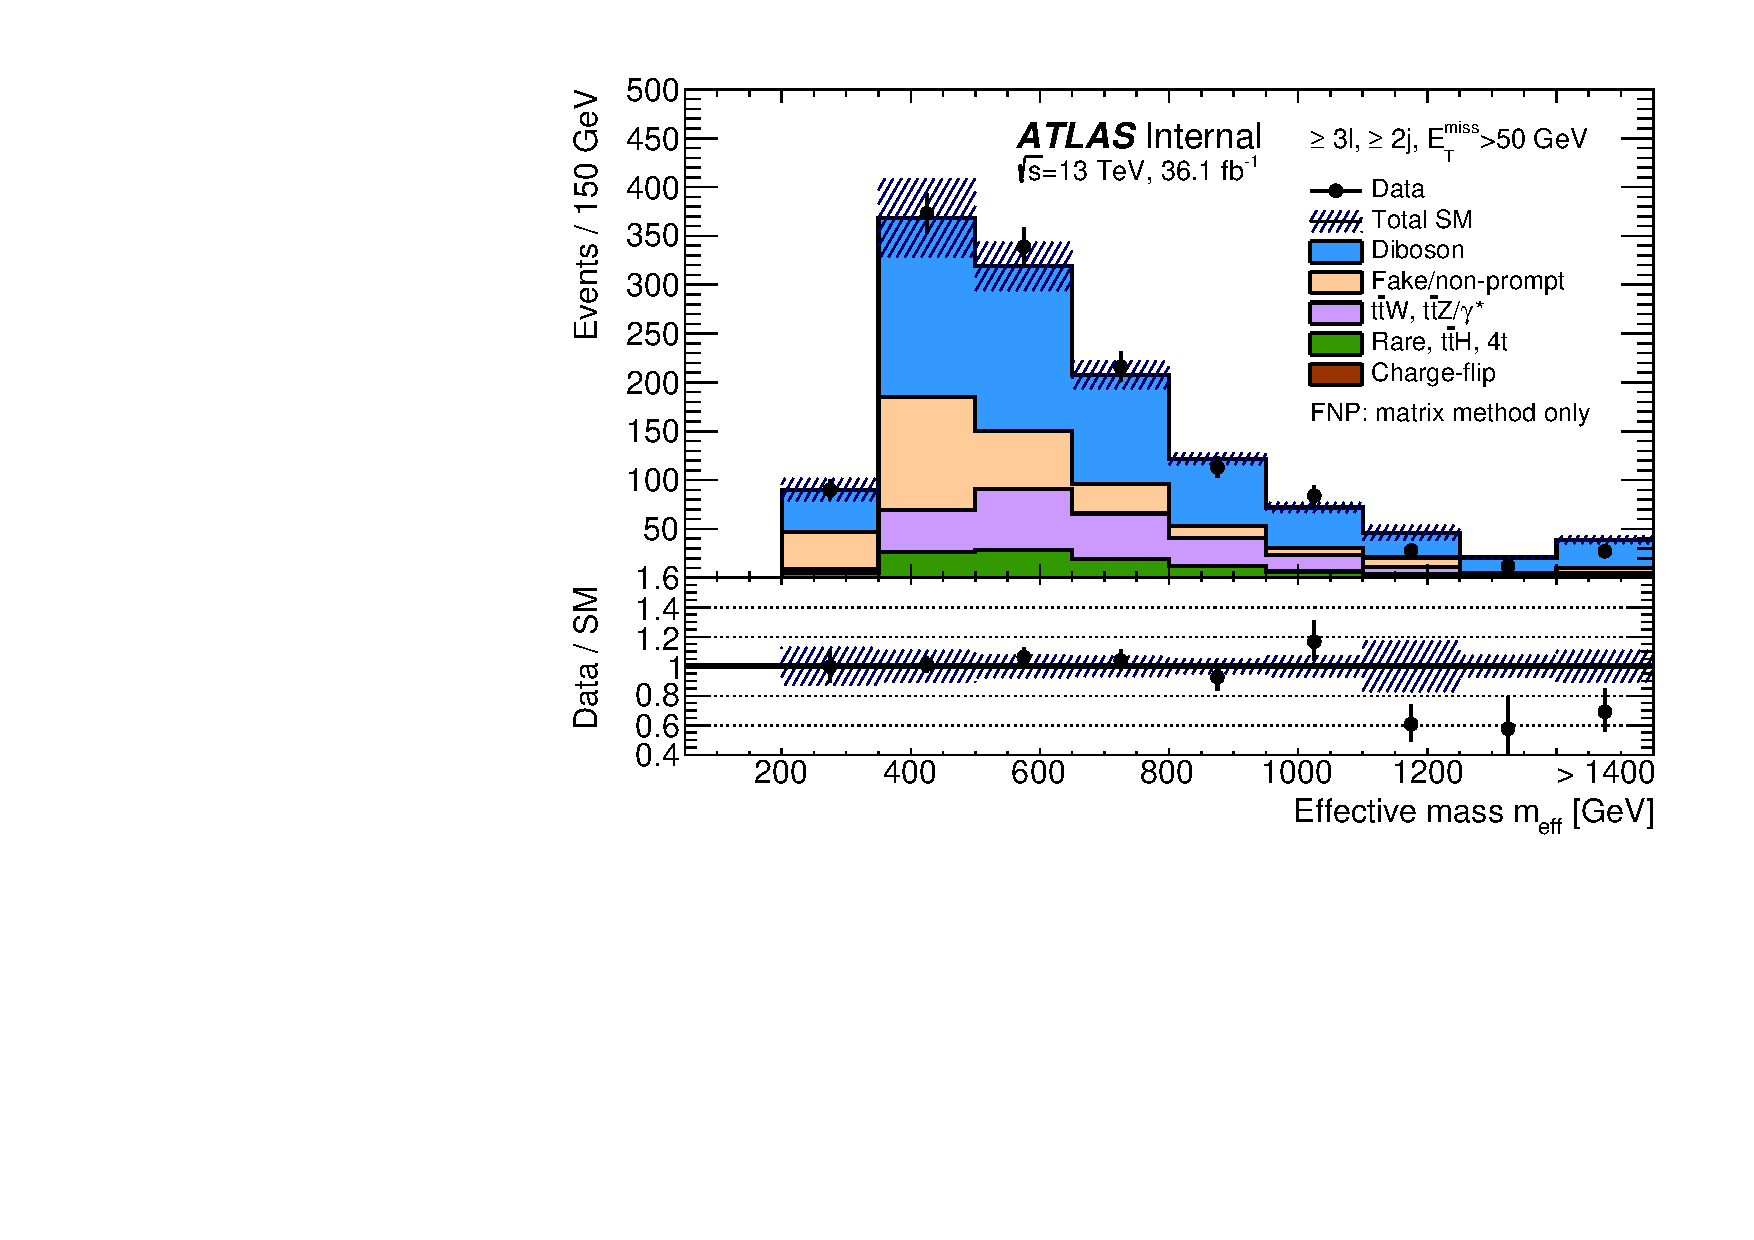
\includegraphics[width=\textwidth]{PAPER_TRILEP_2JMET50_meff}\caption{}\label{fig:VRmeff2}\end{subfigure}
\caption{
Distributions of (a) the number of jets, (b) the number of $b$-tagged jets and (c), (d) the effective mass. The distributions are made 
after requiring at least two jets ($\pT>40 \GeV$) and $\met>50 \GeV$, as well as at least two same-sign leptons ((a), (b), (c)) 
or three leptons (d). The uncertainty bands include the statistical uncertainties for the background prediction as well as the 
systematic uncertainties for fake- or non-prompt-lepton backgrounds (using the matrix method) and charge-flip electrons. Not included
are theoretical uncertainties in the irreducible background contributions.
The rare category is defined in the text.}
\label{fig:Bkg_distribs} 
\end{figure} 

Figure~\ref{fig:VR1b2j} shows a comparison between the estimates of the 
MC template method and the matrix method in a loose selection.

\begin{figure}[htb!]
\begin{subfigure}[t]{0.49\textwidth}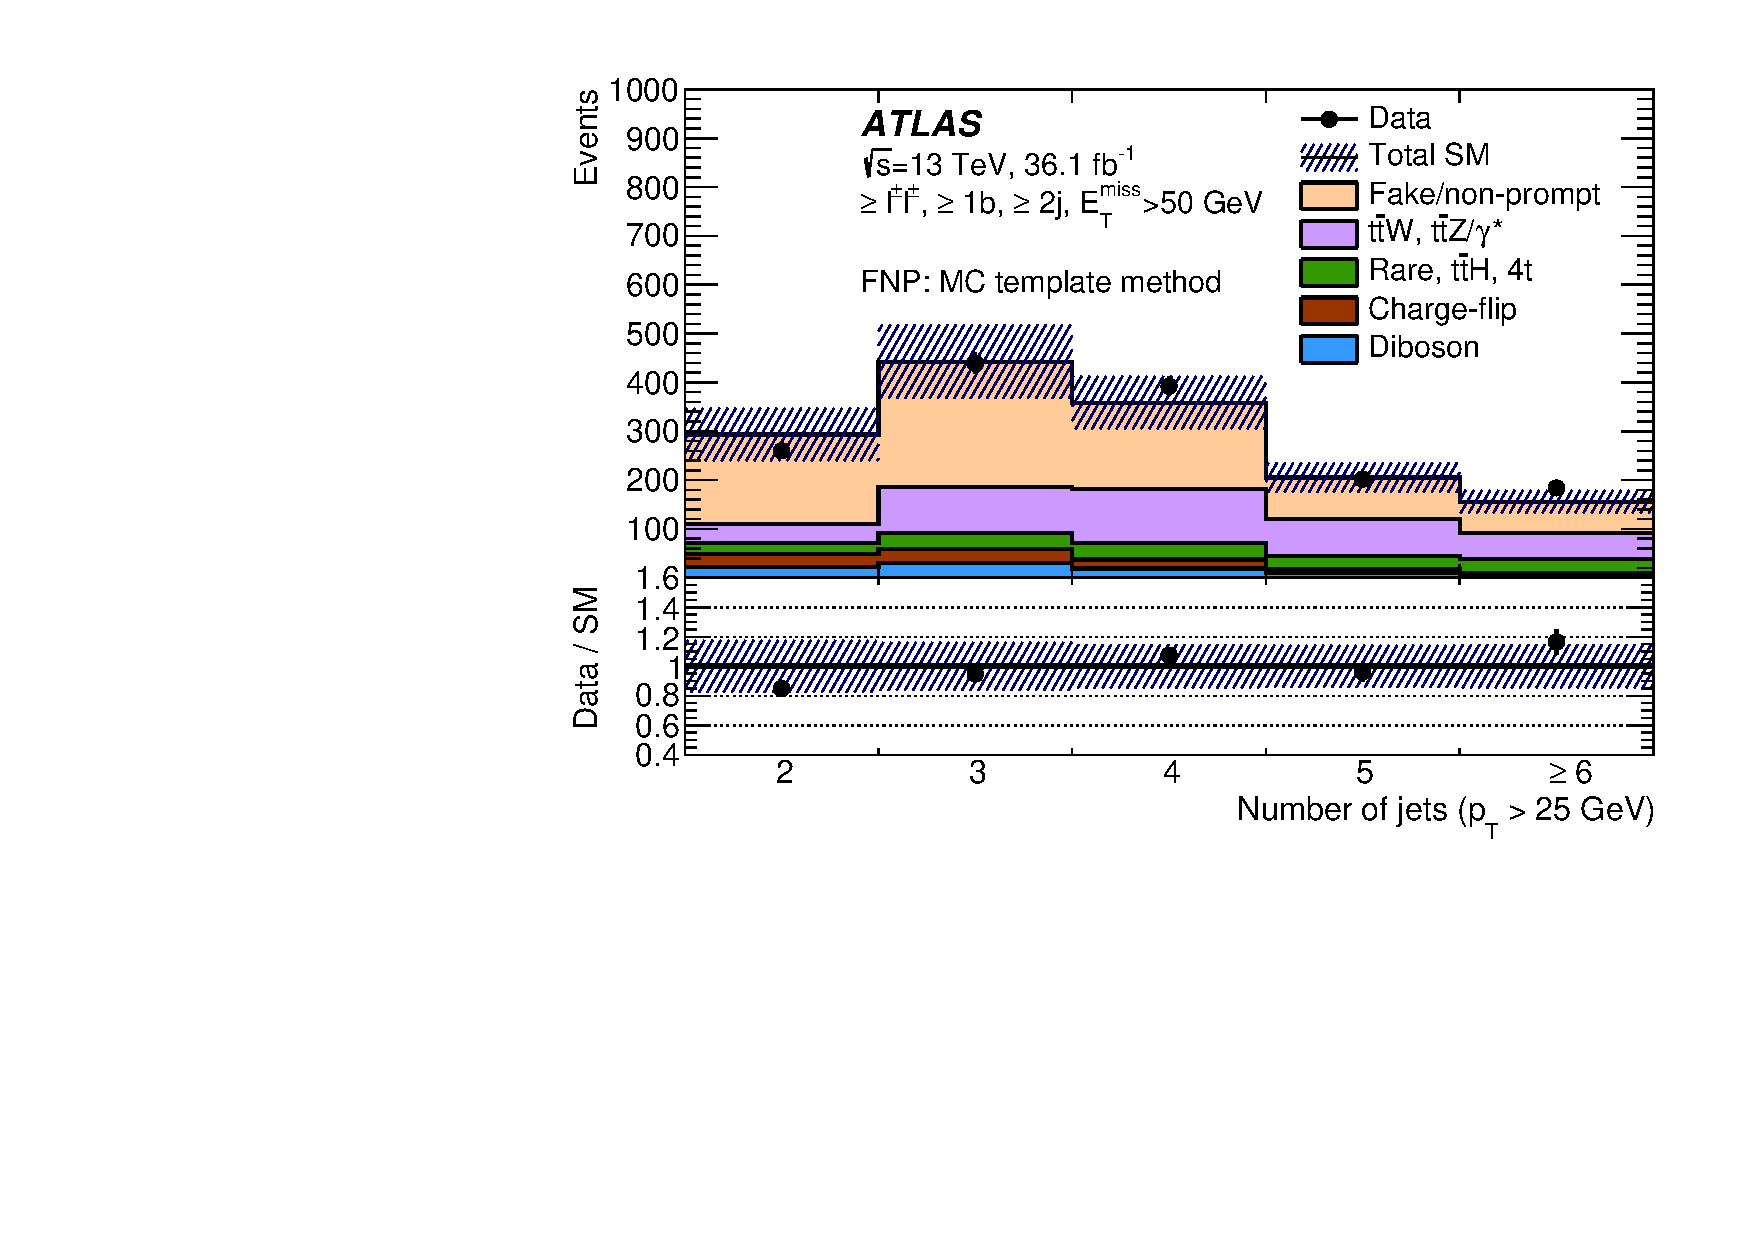
\includegraphics[width=\textwidth]{PAPER_DILEP_1B2JMET50_njets25_template}\caption{}\label{fig:VR1b2j_MxM}\end{subfigure}
\begin{subfigure}[t]{0.49\textwidth}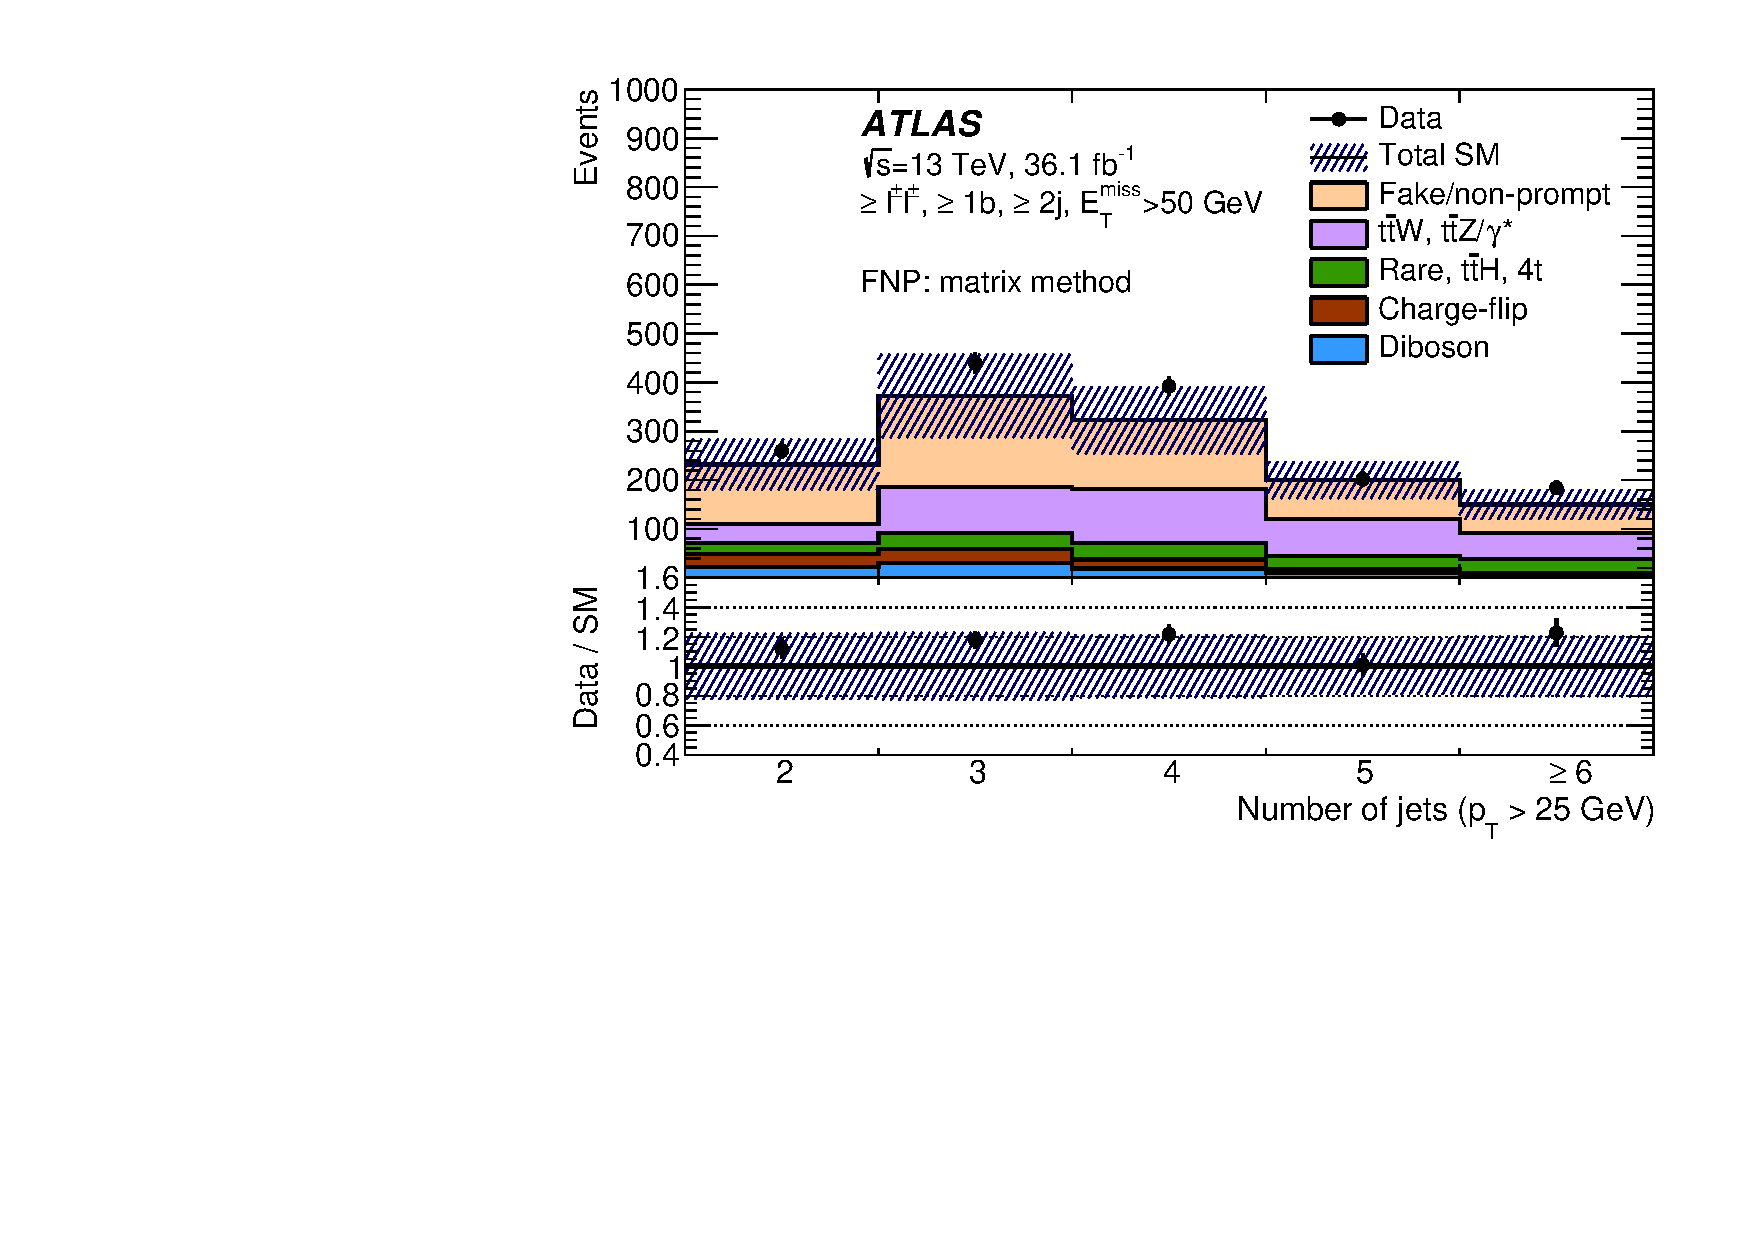
\includegraphics[width=\textwidth]{PAPER_DILEP_1B2JMET50_njets25_matrix}\caption{}\label{fig:VR1b2j_MCT}\end{subfigure}
\caption{
Distributions of the number of jets after requiring at least two jets ($\pT> 40 \GeV$) and $\met> 50 \GeV$, 
as well as at least two same-sign leptons. 
The fake or non-prompt leptons backgrounds are estimated alternatively with the MC template method (\ref{fig:VR1b2j_MCT}) or the matrix method (\ref{fig:VR1b2j_MxM}). 
The uncertainty band includes the statistical uncertainties for the background prediction as well as the
full systematic uncertainties for fake or non-prompt leptons backgrounds or charge-flip electrons. 
The rare category is defined in the text. In both figures, the last bin contains the overflow.
}
\label{fig:VR1b2j}
\end{figure}

Several other distributions with events satisfying the signal region 
requirements except the \met\ cut are shown in 
Figure~\ref{fig:results_datamc_rpc} comparing the two methods. 

\begin{figure}[htb!]
\begin{subfigure}[t]{0.49\textwidth}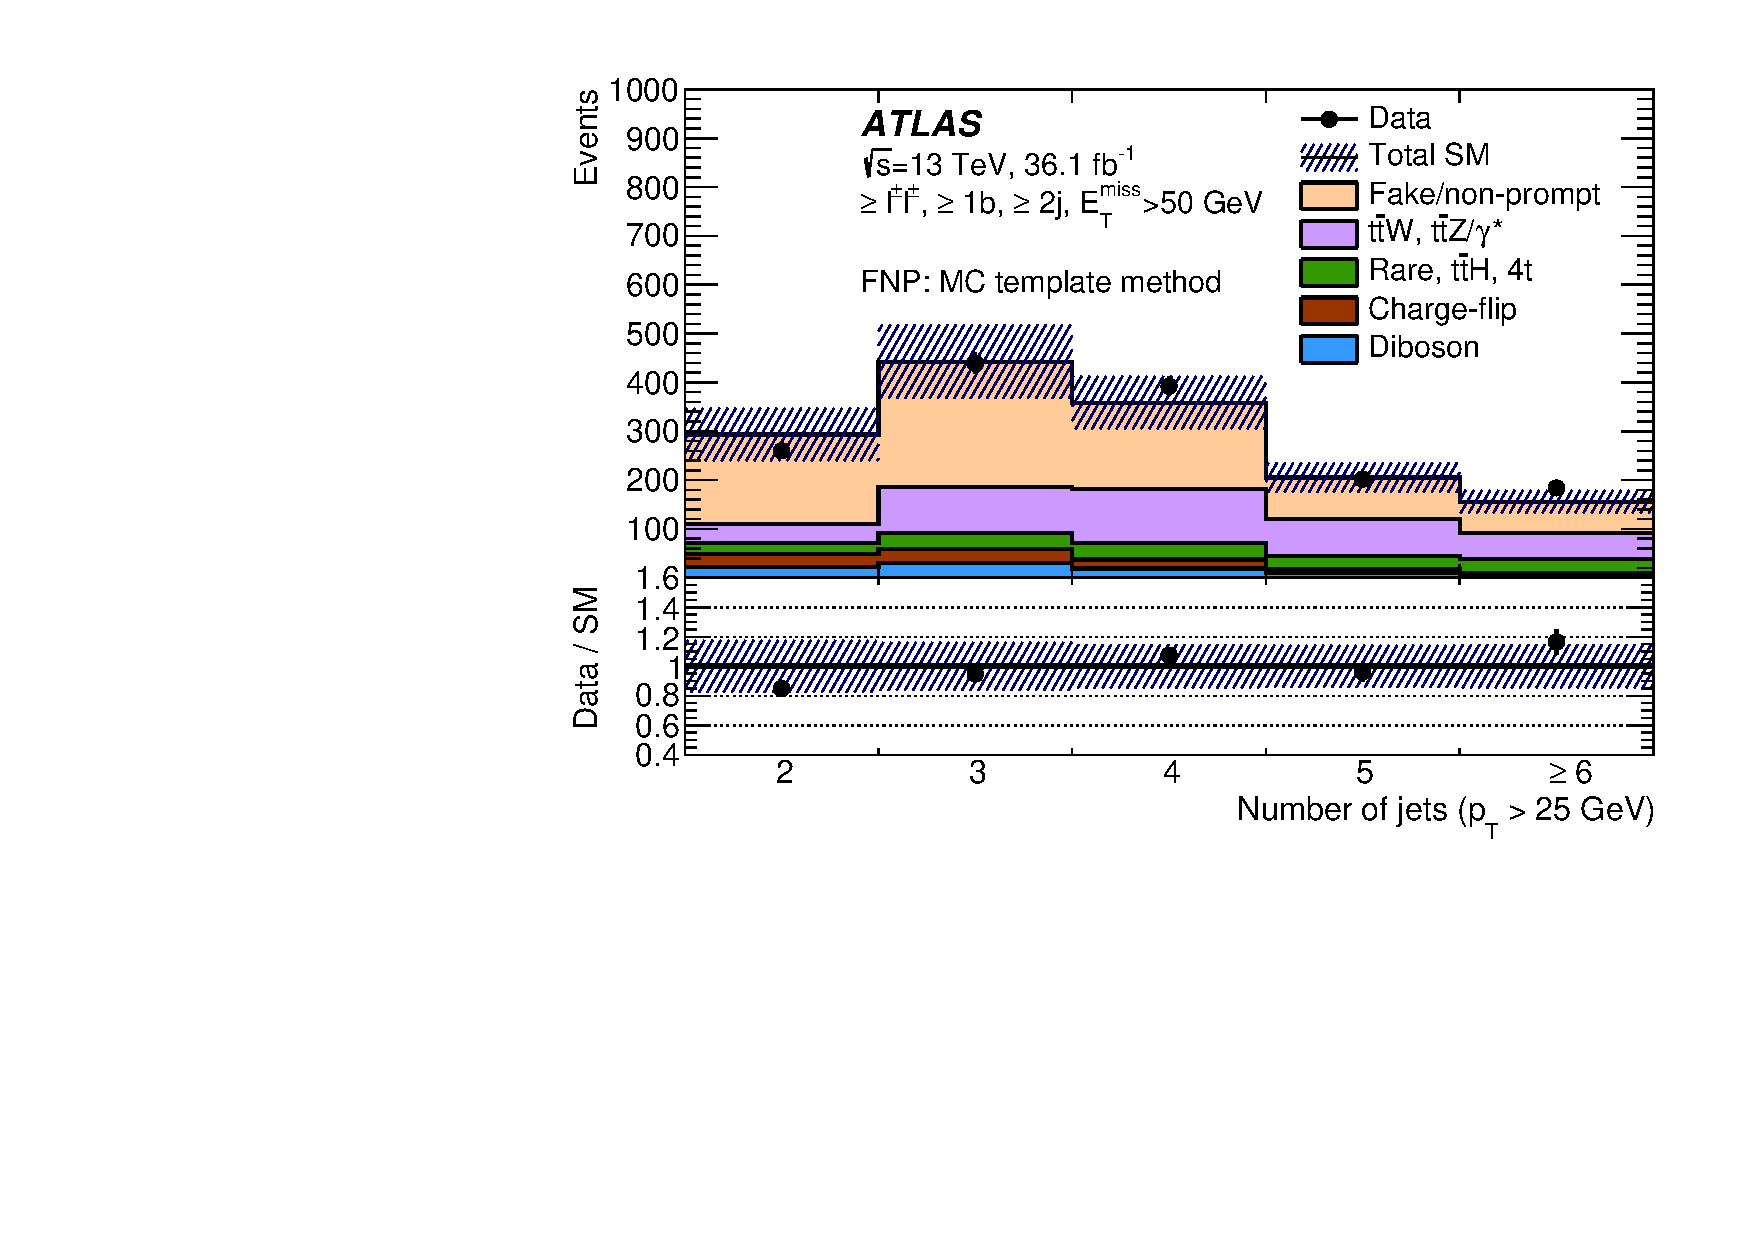
\includegraphics[width=\textwidth]{PAPER_DILEP_1B2JMET50_njets25_template}\caption{}\label{fig:VR1b2j_MxM}\end{subfigure}
\begin{subfigure}[t]{0.49\textwidth}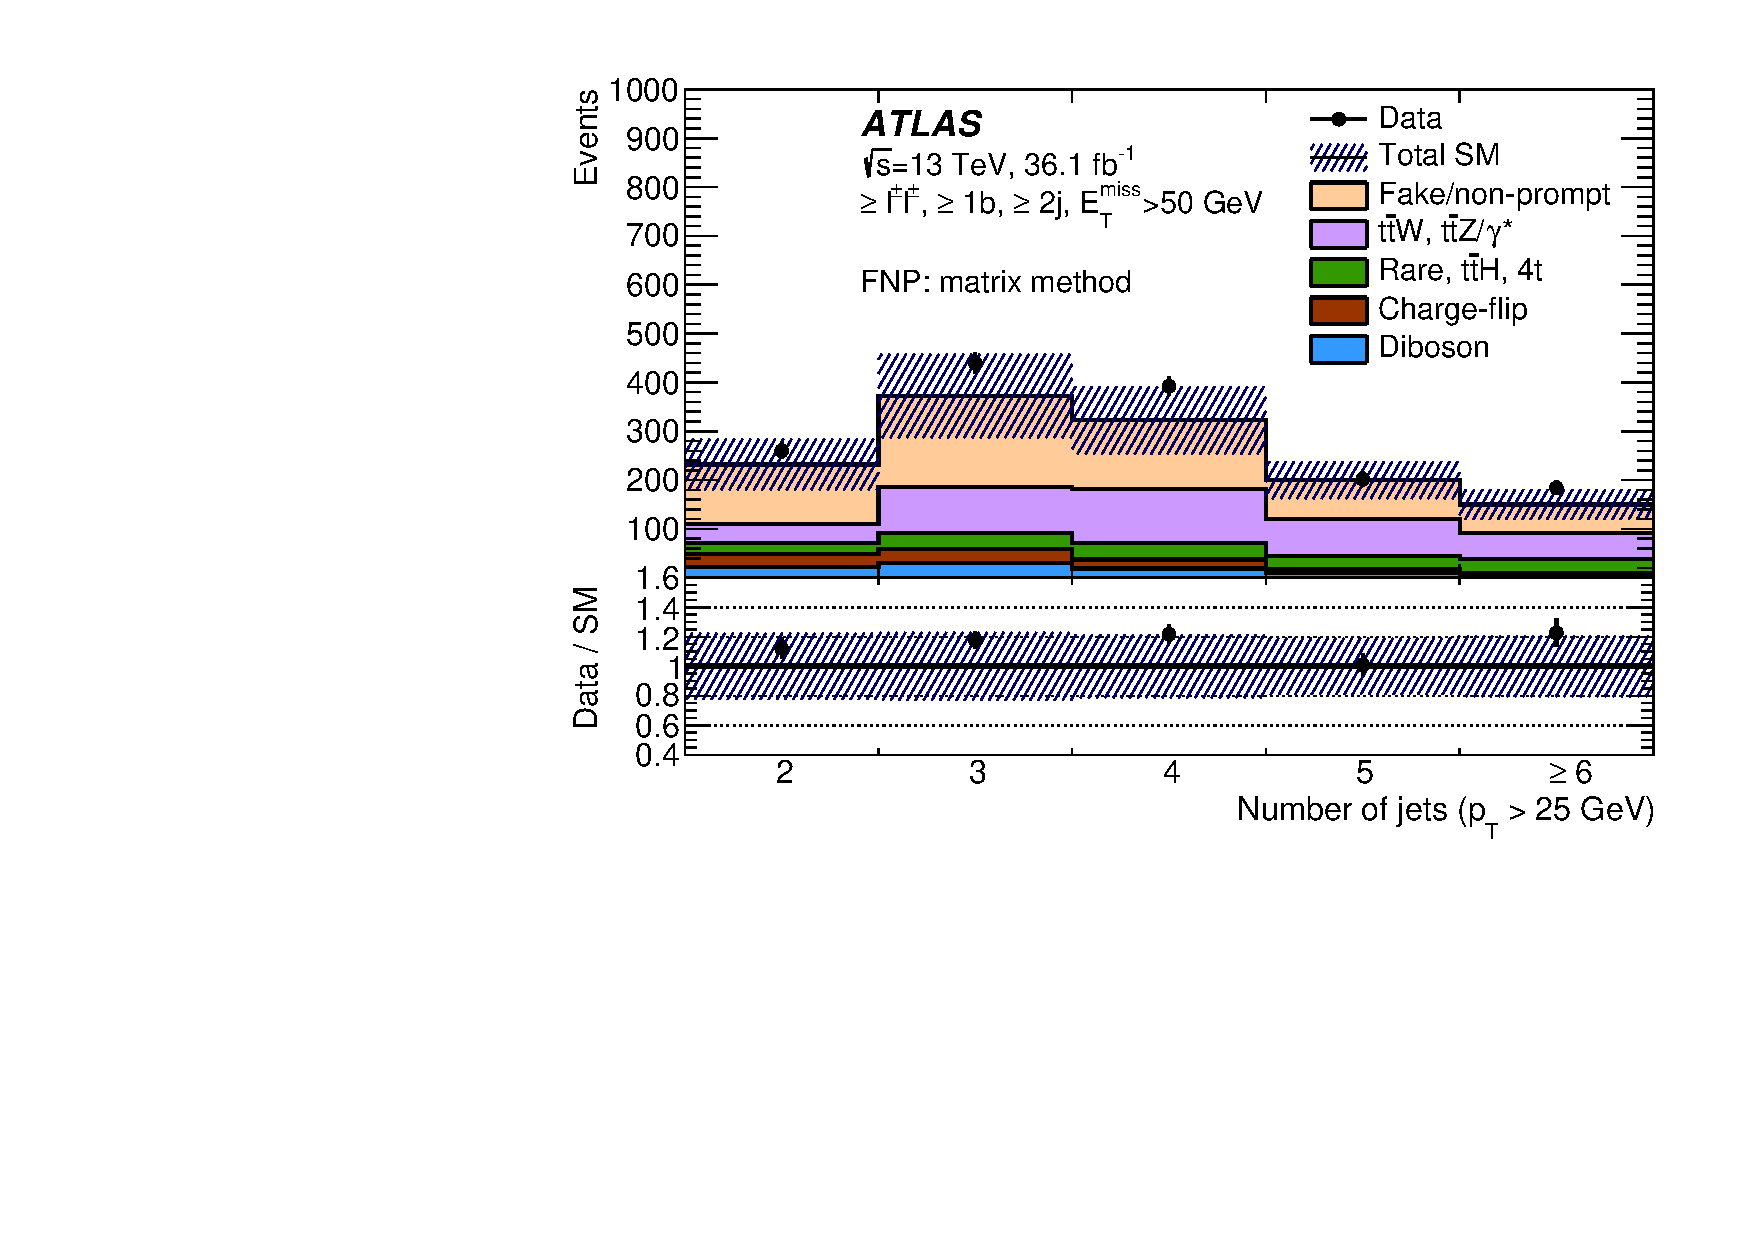
\includegraphics[width=\textwidth]{PAPER_DILEP_1B2JMET50_njets25_matrix}\caption{}\label{fig:VR1b2j_MCT}\end{subfigure}
\caption{
Distributions of (a) the number of jets, (b) the number of $b$-tagged jets and (c), (d) the effective mass. The distributions are made 
after requiring at least two jets ($\pT>40 \GeV$) and $\met>50 \GeV$, as well as at least two same-sign leptons ((a), (b), (c)) 
or three leptons (d). The uncertainty bands include the statistical uncertainties for the background prediction as well as the 
systematic uncertainties for fake- or non-prompt-lepton backgrounds (using the matrix method) and charge-flip electrons. Not included
are theoretical uncertainties in the irreducible background contributions.
The rare category is defined in the text.}
\label{fig:Bkg_distribs} 
\end{figure} 



